\lstset{ %
  backgroundcolor=\color{white},   % choose the background color; you must add \usepackage{color} or \usepackage{xcolor}
  basicstyle=\footnotesize,             % the size of the fonts that are used for the code
  breakatwhitespace=false,            % sets if automatic breaks should only happen at whitespace
  breaklines=true,                 	   % sets automatic line breaking
  captionpos=b,                    	   % sets the caption-position to bottom
  commentstyle=\color{dkgreen},   % comment style
  deletekeywords={...},            	   % if you want to delete keywords from the given language
  escapeinside={\%*}{*)},             % if you want to add LaTeX within your code
  extendedchars=true,                    % lets you use non-ASCII characters; for 8-bits encodings only, does not work with UTF-8
  frame=single,	                        % adds a frame around the code
  keepspaces=true,                         % keeps spaces in text, useful for keeping indentation of code (possibly needs columns=flexible)
  keywordstyle=\color{blue},          % keyword style
  otherkeywords={*,...},                % if you want to add more keywords to the set
  numbers=left,                               % where to put the line-numbers; possible values are (none, left, right)
  numbersep=5pt,                           % how far the line-numbers are from the code
  numberstyle=\tiny\color{gray},   % the style that is used for the line-numbers
  rulecolor=\color{black},                % if not set, the frame-color may be changed on line-breaks within not-black text (e.g. comments (green here))
  showspaces=false,                       % show spaces everywhere adding particular underscores; it overrides 'showstringspaces'
  showstringspaces=false,              % underline spaces within strings only
  showtabs=false,                           % show tabs within strings adding particular underscores
  stepnumber=1,                             % the step between two line-numbers. If it's 1, each line will be numbered
  stringstyle=\color{mauve},          % string literal style
  tabsize=2,	                                  % sets default tabsize to 2 spaces
  title=\lstname                               % show the filename of files included with \lstinputlisting; also try caption instead of title
}

\chapter{Musiksequenzen mit Hilfe von DL4J erzeugen (unfinished)}
{
Dieses Kapitel befasst sich mit der Umsetzung eines LSTM-Netzwerkes, welches anhand einer gegebenen Beispielmusik Musiksequenzen generiert und dessen Implementierung in Deep-Learning4J (DL4J). Als Musikformat wurden MIDI-Dateien gew"ahlt und es wurden zwei Ans"atze zur Verwaltung und Benutzung der Daten verfolgt.

Aufgeteilt ist dieses Kapitel in die Bereiche Eingabe, Netzwerk, Ausgabe und m"ogliche Erweiterungen und Verbesserungen.
Aufteilung:
- Die Eingabe: - Was sind MIDI-Dateien, einlesen und Varianten, DataSets erstellen Varianten\\
- Das Netz: Netzaufbau der 2 Varianten\\
- Die Ausgabe: Ermittlung der Netzausgabe, Umwandlung/Schreiben in MIDI-Datei, Ergebnisse\\
- M"ogliche Erweiterungen und Verbesserungen


\section{Die Eingabe (unfinished)}

\subsection{Was sind MIDI-Dateien?}
Das Musical Instrument Digital Interface (MIDI) Format wird zum Speichern von Audiodateien benutzt. Im Gegensatz zu anderen Formaten enth"allt eine MIDI-Datei eine Liste von Ereignissen, die zum Beispiel von einer Soundkarte in entsprechende T"one umgewandelt werden k"onnen. 
\begin{quote}{\glqq}Dadurch sind die MIDI-Dateien sehr viel kleiner als digitale Audiodateien, und die Ereignisse und Kl"ange sind editierbar, wodurch die Musik neu arrangiert, editiert und interaktiv Komponiert werden kann.{\grqq} - - - \cite{ITwissen}\end{quote} 
MIDI Ereignisse k"onnen als Nachrichten ausgelesen werden. Abbildung 4.1 zeigt den Aufbau so einer Nachricht, welche aus zwei Teilen, Status und Daten, besteht. Das Statusbyte beginnt immer mit einer 1, gefolgt von drei Bits, die die Art der Nachricht enthalten (in Abbildung 4.1 mit s gekennzeichnet). Die letzten vier Bits geben einen von 16 m"oglichen Kan"alen an (in Abbildung 4.1 mit n gekennzeichnett).
Die Datenbytes beginnen immer mit einer 0 und geben somit Raum f"ur 128  m"ogliche Werte.
\renewcommand{\figurename}{Abb.}
\begin{figure}[htp]
\centering
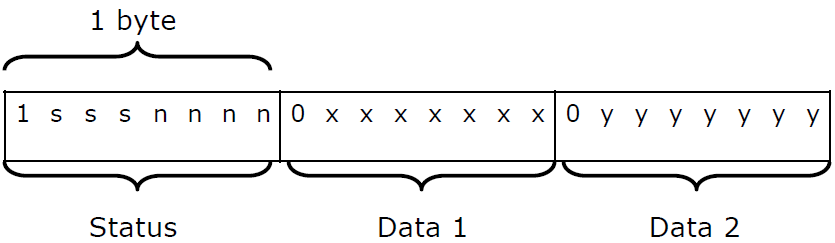
\includegraphics[width=0.60\textwidth]{pictures/MIDI-Message.png}
\caption[MIDI Nachricht]{MIDI Nachricht (Quelle: \cite{MIDIImg})}
\end{figure}

Tabelle \ref{tbl:midiMess} zeigt beispielhaft den Aufbau der Nachrichten {\glqq}Note aus{\grqq} und {\glqq}Note an{\grqq}. Das n im Statusbyte steht f"ur die Kanalnummer, welche Hexadezimal angegeben wird und somit einen Bereich von 0 bis F umfasst. Daten 1 enth"allt eine der 128 m"oglichen Noten und Daten 2 die Geschwindigkeit bzw. die Intensit"at mit der die Note gespielt oder losgelassen wird. Eine {\glqq}Note an{\grqq}-Nachricht mit der Geschwindigkeit 0 ist gleichbedeutend zu {\glqq}Note aus{\grqq}.
(\cite{MIDI})

\begin{table} [h]
\centering
%%\begin{tabular}{|p{0.8cm}|p{3.7cm}|p{8.8cm}|p{8.8cm}|}\hline
\begin{tabular}{|c|c|c|c|}\hline
   \textbf{Nachricht} & \textbf{Status} & \textbf{Daten 1} & \textbf{Daten 2}\\ \hline
   Note aus & 8n & Notennummer & Geschwindigkeit \\ \hline
   Note an & 9n & Notennummer & Geschwindigkeit \\ \hline
 \end{tabular}
\caption{MIDI Nachrichtenformat}
\label{tbl:midiMess} % Verweis im Text mittels \ref{tbl:midiMess}
\end{table}


\subsection{MIDI-Dateien lesen (unfinished)}
- einlesen eines MIDI Files
- Vernachl"assigung des MIDI-Takts (zur Komplexit"atsverkleinerung)

\subsubsection{Variante 1: Ereignissmatrix (unfinished) }
...Quellcode \ref{lst:midiEvents}
\lstinputlisting[language=JAVA, firstline=1, lastline=5,  captionpos=b, caption={MidiEvents Konstruktor}, label=lst:midiEvents]
{code_snippets/midiEvents_auszug.java}
Quellcode \ref{lst:matrixValidData}
\lstinputlisting[language=JAVA, firstline=20, lastline=30,  captionpos=b, caption={Ereignissmatrix: Listen von g"ultigen Daten}, label=lst:matrixValidData]
{code_snippets/app_auszug.java}

\subsubsection{Variante 2: Ereignissschl"ussel (unfinished) }
...
Event -> String -> Integer
Tabelle \ref{tbl:eventKey}
\begin{table} [h]
\centering
%%\begin{tabular}{|p{0.8cm}|p{3.7cm}|p{8.8cm}|p{8.8cm}|}\hline
\begin{tabular}{|c|c|c|c|c|}\hline
   & \textbf{Kanalnummer} & \textbf{Ereignistyp} & \textbf{Notennummer} & \textbf{Geschwindigkeit}\\ \hline
  \textbf{Stellen} & nn & n & nnn & nnn \\ \hline
  \textbf{Beispiel} & 00 & 1 & 081 & 064 \\ \hline
 \end{tabular}
\caption{Ereignissschl"ussel}
\label{tbl:eventKey}
\end{table}
Quellcode \ref{lst:matrixValidData}
\lstinputlisting[language=JAVA, firstline=9, lastline=13,  captionpos=b, caption={Ereignissschl"ussel: Liste von g"ultigen Daten}, label=lst:matrixValidData]
{code_snippets/app_auszug.java}

\subsection{DataSets erstellen (unfinished)}
- 2 Varianten implementiert (Eventschl"ussel und Eventmatrix)
- umwandeln der eingelesenen MIDI-Events

\subsubsection{Variante 1: Ereignissmatrix (unfinished) }
...Quellcode \ref{lst:matrixData} schon hier h"atte auffallen m"ussen dass das nicht funktioniert
- f"ur Backpropagation muss INDArray 3-D sein
\lstinputlisting[language=JAVA, firstline=2, lastline=23,  captionpos=b, caption={Ereignissmatrix: Trainingsdaten}, label=lst:matrixData]
{code_snippets/LSTMNetwork_auszug.java}

\subsubsection{Variante 2: Ereignissschl"ussel (unfinished) }
...Quellcode \ref{lst:schlusselData}
\lstinputlisting[language=JAVA, firstline=26, lastline=43,  captionpos=b, caption={Ereignissschl"ussel: Trainingsdaten}, label=lst:schlusselData]
{code_snippets/LSTMNetwork_auszug.java}




\section{Das Netzwerk (unfinished)}
- 1 HiddenLayer
\subsubsection{Variante 1: Ereignissmatrix (unfinished) }
Layergr"o{\ss}en
Quellcode \ref{lst:matrixLayer}
\lstinputlisting[language=JAVA, firstline=32, lastline=33,  captionpos=b, caption={Ereignissmatrix: Gr"o{\ss}e der Ein- und Ausgangslayer}, label=lst:matrixLayer]
{code_snippets/app_auszug.java}
...

\subsubsection{Variante 2: Ereignissschl"ussel (unfinished) }
Layergr"o{\ss}en
Quellcode \ref{lst:schlusselLayer}
\lstinputlisting[language=JAVA, firstline=15, lastline=16,  captionpos=b, caption={Ereignissschl"ussel: Gr"o{\ss}e der Ein- und Ausgangslayer}, label=lst:schlusselLayer]
{code_snippets/app_auszug.java}
...
Version 1: Yiruma track2 = 1040 events, 36 in/output M"oglichkeiten, hidden = in*2 -> zu wenig varianz, lernt eine Note zu spielen
Version 1: F"ur Elise track2 = 1254 events, 417 in/output M"oglichkeiten, hidden = in*2 (hidden = in) -> netz lernt nicht
Version 1: Bumblebee track1 = 2620 events, 1053 in/output M"oglichkeiten, hidden = in*2 (hidden = in) -> out of memory, can not allocate




\section{Die Ausgabe (unfinished)}
\subsection{Auswerten der Netzwerkausgabe (unfinished)}
\subsubsection{Variante 1: Ereignissmatrix (unfinished)}
...
...Quellcode \ref{lst:matrixOutput}
\lstinputlisting[language=JAVA, firstline=48, lastline=63,  captionpos=b, caption={Ereignissmatrix: Netzausgabe}, label=lst:matrixOutput]
{code_snippets/LSTMNetwork_auszug.java}

\subsubsection{Variante 2: Ereignissschl"ussel (unfinished)}
...
...Quellcode \ref{lst:schlusselOutput}
\lstinputlisting[language=JAVA, firstline=66, lastline=81,  captionpos=b, caption={Ereignissschl"ussel: Netzausgabe}, label=lst:schlusselOutput]
{code_snippets/LSTMNetwork_auszug.java}


\subsection{MIDI Files schreiben (unfinished)}
...

\subsection{Ergebnisse (unfinished)}
- did not have the time nor computational power to experiment further with this
- nur Variante 2, da Variante 1 fehlerhaft ist

\renewcommand{\figurename}{Abb.}
\begin{figure}[htp]
%%\begin{floatingfigure}[r]{textwidth}
\centering
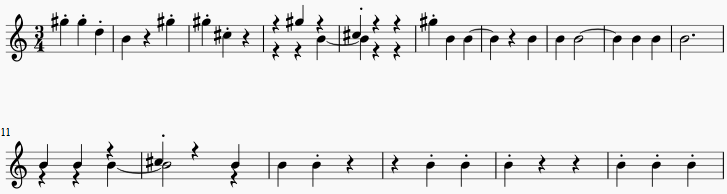
\includegraphics[width=1\textwidth]{pictures/sampleMidi1.png}
\caption[Beispiel Ausgabe 1]{Beispiel Ausgabe 1}
%%\end{floatingfigure} 
\end{figure}

\renewcommand{\figurename}{Abb.}
\begin{figure}[htp]
%%\begin{floatingfigure}[r]{textwidth}
\centering
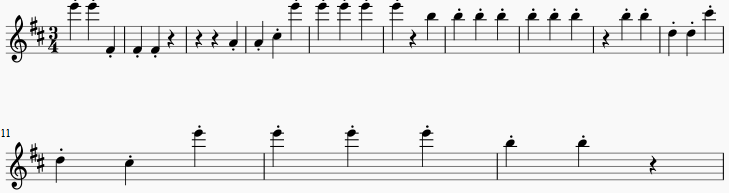
\includegraphics[width=1\textwidth]{pictures/sampleMidi2.png}
\caption[Beispiel Ausgabe 2]{Beispiel Ausgabe 2}
%%\end{floatingfigure} 
\end{figure}

\section{M"ogliche Erweiterungen und Verbesserungen (unfinished)}
- DataSetIterator()
} %% Ende Chapter{Musiksequenzen mit Hilfe von DL4J erzeugen}